\documentclass[12pt]{article}
\usepackage[a4paper, portrait, margin=1cm, right=1cm]{geometry}
\usepackage{fontspec}
\usepackage{graphicx}
\usepackage[fleqn]{amsmath}
\usepackage{setspace}
\usepackage{mathtools}
\usepackage{indentfirst}

\graphicspath{./graphics/}
\setmainfont[Ligatures=TeX]{Linux Libertine}

\title{Информационные технологии. Лекция 07. Групповое взаимодействие}
\author{Студент группы 2305 Макурин Александр}
\date{03 апреля 2023}
\begin{document}
\maketitle
Взаимодействие двух систем: \\
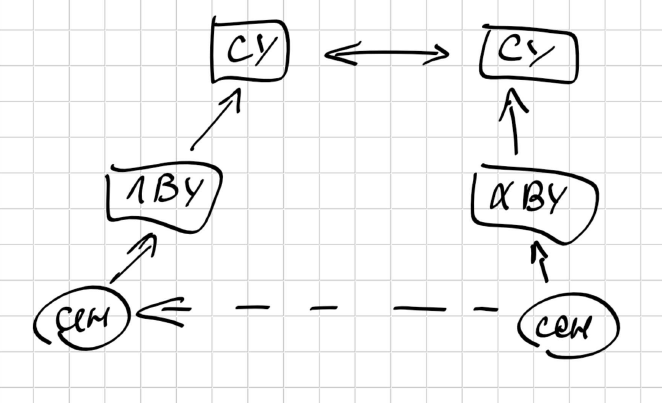
\includegraphics[width=0.5\textwidth]{graphics/pic01.png}

В более тривиальном случае (марсоход/типичный беспилотник): \\

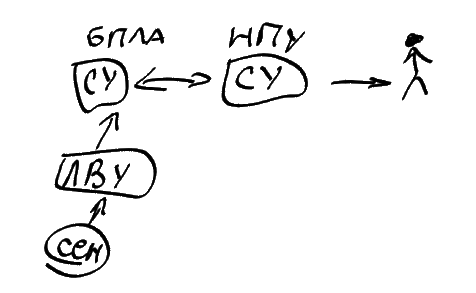
\includegraphics[width=0.5\textwidth]{graphics/pic02.png}

\[
    \begin{cases}
        TK^C_E \rightarrow max \\
        cost_{e_i}(TK_{e_i}^C) \leq r_{e_i}
    \end{cases}
\]
\[
    TK_E^C = \cup TK_{e_i}^C
\]
\[
    Env \xrightarrow{Act} Env^{TK}
\]
Среда переходит в дрегое состояние. Два вариента задания группы:
\begin{enumerate}
    \item $Env = \text{const}, \ Env_i \simeq Env_j$ \\
          $S_{Env} = \Phi(E^T, Env_i) + \int_{0}^{T}F(E^T, Act, Env^0)dt$\\
          $\Phi$ — функция, описывающая влияние системы на $Env$ ($\sim Env^T \backslash S_E$). $\int_{0}^{T}F(E^T, Act, Env^0)dt$ — состояние системы ($\sim S_E$) или функционал ($y$).
    \item $Env \neq \text{const}, \ Env_i = f(Env_{i - 1}, O)$, $O$ — возмущения. \\
          $S = \Phi(E^T, Env^0, O^t) + \int_{0}^{T}F(E^T, Act, Env^0, O^T)dt$
\end{enumerate}

\[
    \begin{cases}
        y \rightarrow max \\
        cost \leq R
    \end{cases}
    \Rightarrow
    \begin{aligned}
        \text{Без возмущений: } \begin{cases}
                                    Env \rightarrow Env^{TK} \\
                                    cost \leq R
                                \end{cases} \\
        \text{С возмущениями: } \begin{cases}
                                    Env(0) \rightarrow^{TK}(0) \\
                                    cost \leq R
                                \end{cases}
    \end{aligned}
\]

\section{Методы управления (МУ)}
$T$ — сложность.
$N$ — количество элементов.

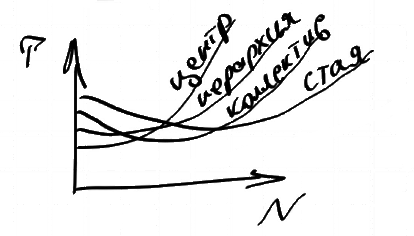
\includegraphics[width=0.5\textwidth]{graphics/pic03.png}

\subsection{Единоначальный МУ}
Пример — диктатура. Плюс — если $N \rightarrow 0$, то $T \rightarrow 0$ и $T_{Env^{TK}} \rightarrow 0$ (время изменения среды).
\subsection{Иерархический МУ}
\subsection{Коллективный МУ}
Пример — косяк рыб. Есть выборный лидер, который периодически меняется.
\subsection{Стайный (роевой) МУ}
В чистом виде в природе не существует

\subsection*{Трудности группового взаимодействия:}
\begin{itemize}
    \item Разделение задач
    \item Субъективность восприятия
    \item Субъективность развития
\end{itemize}

Ad-hoc система — система, способная к горячей замене элементов.
Manet — $\pm$ статичная Ad-hoc.
Vanet — более динамичная Manet.

\section{Распределение задач}
$G = {g_1, .., g_i}$ — цели группы.

$Y_i^l$ — цена достижения цели $l$ роботом $i$.

$Y_i^{max}$ — максимально возможное приращение функционала роботом.

$d_i^l = \dfrac{\Delta Y_i}{\Delta Y_i^{max}}$

$Y_{all} = \sum_{i = 1}^{N} \sum_{l = 1}^{L}d_i^l \rightarrow max$

$y_{max} : TK^R = 0$

Мы всегда стремимся к максимуму функционала.

Таблица — если привязываем элементы к типу задачи.

Усложнённый пример — все элементы равноценны.

Полный перербор — при всей полноте информации (роботы передают всю информацию между собой).

\subsection{Аукцион}
Есть аукционер (один из элементов ($e_i$)), который выбирает кому какую задачу выполнить.

\begin{enumerate}
    \item $e_j \in E \backslash \{e_i\}$, $j \pm i : d_j^l$ — затраты
    \item $j = \arg \min \{d_j^l\}$
\end{enumerate}

\subsection{Опорный план}
Получаемый план неоптимален, зато процесс его получения быстрый.

\begin{enumerate}
    \setcounter{enumi}{-1}
    \item $e_i : \{d_i^l\}$
    \item $l = i$ или случайным образом
    \item $<TK, R_i>$ — опорный план
    \item сравниваем для кого дешевле — попарное сравнение $d_i^l - d_j^l \leq 0 \Rightarrow e_i$ остаётся на задаче.
\end{enumerate}

\subsection{Итеративное улучшение}
\begin{enumerate}
    \item Выбор наилучшего варианта (по функционалу)
    \item Обмен информацией
    \item Выбор улучшенного варианта
    \item Назад к пункту два пока план меняется
\end{enumerate}

Формально:
\begin{enumerate}
    \setcounter{enumi}{-1}
    \item $l = \arg \min \{d_i^l\}$ для каждого $e_i \in E \Rightarrow <e_i, tR>$
    \item $d_i^l - d_j^l \leq 0 \Rightarrow e_i$ остаётся на задаче.
\end{enumerate}

Для БТС функционал может быть выражен исходя из затрат или преимуществ.
\end{document}